% Copyright 2021 Politecnico di Milano, Italy. Inc. All rights reserved.

\documentclass[11pt,a4paper,twocolumn]{article}

% === Packages and configurations ===
% Titles
\usepackage{titlesec}
\usepackage{color}

% Language and fonts
\usepackage[utf8]{inputenc}
\usepackage[english]{babel}
\usepackage[T1]{fontenc} % Font encoding

% Images
\usepackage{graphicx}
\graphicspath{{Images/}} % Path for images' folder
\usepackage{eso-pic} % For the background picture on the title page
\usepackage{subfig} % Numbered and caption subfigures using \subfloat
\usepackage[font=footnotesize]{caption} % Coloured captions
\usepackage{transparent}

% Math
\usepackage{amsmath}
\usepackage{amsthm}
\usepackage{bm}
\usepackage[overload]{empheq}  % For braced-style systems of equations

% Tables
\usepackage{tabularx}

\usepackage{longtable} % tables that can span several pages
\usepackage{colortbl}

% Algorithms
\usepackage{algorithm}
\usepackage{algorithmic}

% Bibliography and references
\usepackage[colorlinks=true,linkcolor=black,anchorcolor=black,citecolor=black,filecolor=black,menucolor=black,runcolor=black,urlcolor=black]{hyperref} % Adds clickable links at references
\usepackage{cleveref}
\usepackage[square, numbers, sort&compress]{natbib} % Square brackets, citing references with numbers, citations sorted by appearance in the text and compressed
\bibliographystyle{plain} % You may use a different style adapted to your field

% Appendix
\usepackage{appendix}

% Bullet lists
\usepackage{enumitem}

% Other
\usepackage{amsthm,thmtools,xcolor} % Coloured "Theorem"
\usepackage{comment} % Comment part of code
\usepackage{fancyhdr} % Fancy headers and footers
\usepackage{lipsum} % Insert dummy text
\usepackage{tcolorbox} % Create coloured boxes (e.g. the one for the key-words)
\usepackage{stfloats} % Correct position of the tables

% === New commands ===
\newcommand{\bea}{\begin{eqnarray}} % Shortcut for equation arrays
\newcommand{\eea}{\end{eqnarray}}
\newcommand{\e}[1]{\times 10^{#1}}  % Powers of 10 notation
\newcommand{\mathbbm}[1]{\text{\usefont{U}{bbm}{m}{n}#1}} % From mathbbm.sty
\newcommand{\pdev}[2]{\frac{\partial#1}{\partial#2}}

% === Title settings ===
% Set the geometric layout of the document
\usepackage{geometry}
\geometry{
  top=3cm,
  left = 1.5cm,
  right = 1.5cm,
  bottom=2cm,
  headheight= 2cm,
  headsep= 0cm,
}
\raggedbottom 

% Create color bluePoli (-> manuale grafica coordinata:  https://www.polimi.it/fileadmin/user_upload/il_Politecnico/grafica-coordinata/2015_05_11_46xy_manuale_grafica_coordinata.pdf)
\definecolor{bluePoli}{cmyk}{0.4,0.1,0,0.4}

% Custom theorem environments
\declaretheoremstyle[
  headfont=\color{bluePoli}\normalfont\bfseries,
  bodyfont=\color{black}\normalfont\itshape,
]{colored}

\captionsetup[figure]{labelfont={color=bluePoli}} % Set colour of the captions
\captionsetup[table]{labelfont={color=bluePoli}} % Set colour of the captions
\captionsetup[algorithm]{labelfont={color=bluePoli}} % Set colour of the captions

\theoremstyle{colored}
\newtheorem{theorem}{Theorem}[section]
\newtheorem{proposition}{Proposition}[section]

% Enhances the features of the standard "table" and "tabular" environments.
\newcommand\T{\rule{0pt}{2.6ex}}
\newcommand\B{\rule[-1.2ex]{0pt}{0pt}}

% Algorithm description
\newcounter{algsubstate}
\renewcommand{\thealgsubstate}{\alph{algsubstate}}
\newenvironment{algsubstates}{
    \setcounter{algsubstate}{0}%
    \renewcommand{\STATE}{%
    \stepcounter{algsubstate}%
    \Statex {\small\thealgsubstate:}\space}
    }{}
    
% Custom theorem environment
\newcolumntype{L}[1]{>{\raggedright\let\newline\\\arraybackslash\hspace{0pt}}m{#1}}
\newcolumntype{C}[1]{>{\centering\let\newline\\\arraybackslash\hspace{0pt}}m{#1}}
\newcolumntype{R}[1]{>{\raggedleft\let\newline\\\arraybackslash\hspace{0pt}}m{#1}}

% Custom itemize environment
\setlist[itemize,1]{label=$\bullet$}
\setlist[itemize,2]{label=$\circ$}
\setlist[itemize,3]{label=$-$}
\setlist{nosep}

% Set separation of columns 
\setlength{\columnsep}{30pt}

% Create command for background pic
\newcommand\BackgroundPic{% Adding background picture
	\put(198,330){
		\parbox[b][\paperheight]{\paperwidth}{%
			\vfill
			\centering
			\transparent{0.4}
			
\includegraphics[width=0.7\paperwidth]{raggiera_polimi.eps}%
			\vfill
}}}

% Set indentation
\setlength\parindent{0pt}

% Custom title commands
\titleformat{\section}
{\color{bluePoli}\normalfont\Large\bfseries}
{\color{bluePoli}\thesection.}{1em}{}
\titlespacing*{\section}
{0pt}{2ex}{1ex}

\titleformat{\subsection}
{\color{bluePoli}\normalfont\large\bfseries}
{\color{bluePoli}\thesubsection.}{1em}{}
\titlespacing*{\subsection}
{0pt}{2ex}{1ex}

% Custom headers and footers
\pagestyle{fancy}
\fancyhf{}
      
\fancyfoot{}
\fancyfoot[C]{\thepage} % page
\renewcommand{\headrulewidth}{0mm} % headrule width
\renewcommand{\footrulewidth}{0mm} % footrule width

\makeatletter
\patchcmd{\headrule}{\hrule}{\color{black}\hrule}{}{} % headrule
\patchcmd{\footrule}{\hrule}{\color{black}\hrule}{}{} % footrule
\makeatother

% -> Create the header
\chead[C]{
\centering
\begin{tcolorbox}[arc=0pt, boxrule=0pt, colback=bluePoli!60, width=\textwidth, colupper=white]
    \textsc{\textbf{Executive summary}} \hfill \textsc{\textbf{\author}} 
\end{tcolorbox}
}

\renewcommand{\title}{Ray Distribution Aware Heuristics for Bounding Volume Hierarchies Construction}
\renewcommand{\author}{Lapo Falcone}
\newcommand{\course}{Computer Science and Engineering}
\newcommand{\advisor}{Prof. Marco Gribaudo}
\newcommand{\YEAR}{2023-24}

% === Start of document ===
\begin{document}

% Title page
% DO NOT REMOVE SPACES BETWEEN LINES!

\twocolumn[{\begin{@twocolumnfalse}

\AddToShipoutPicture*{\BackgroundPic}

\vspace{-1.5cm}
\hspace{-0.6cm}
\includegraphics[width=0.6\textwidth]{logo_polimi_ing_indinf.eps}

\vspace{-1mm}
\fontsize{0.3cm}{0.5cm}\selectfont \bfseries \textsc{\color{bluePoli} Executive Summary of the Thesis}\\

\vspace{-0.2cm}
\Large{\textbf{\color{bluePoli}{\title}}}\\

\vspace{-0.2cm}
\fontsize{0.3cm}{0.5cm}\selectfont \bfseries \textsc{\color{bluePoli} Laurea Magistrale in \course}\\

\vspace{-0.2cm}
\fontsize{0.3cm}{0.5cm} \normalfont Author: \textsc{\textbf{\author}} \hspace{1cm}
\fontsize{0.3cm}{0.5cm} \normalfont Advisor: \textsc{\textbf{\advisor}} \hspace{1cm}
\fontsize{0.3cm}{0.5cm} \normalfont Academic year: \textsc{\textbf{\YEAR}}

\small \normalfont

\vspace{11pt}

\centerline{\rule{1.0\textwidth}{0.4pt}}

\vspace{15pt}
\end{@twocolumnfalse}}]

\thispagestyle{plain} % In order to not show the header in the first page

\AddToShipoutPicture{%
	\put(0.5\paperwidth-18,21){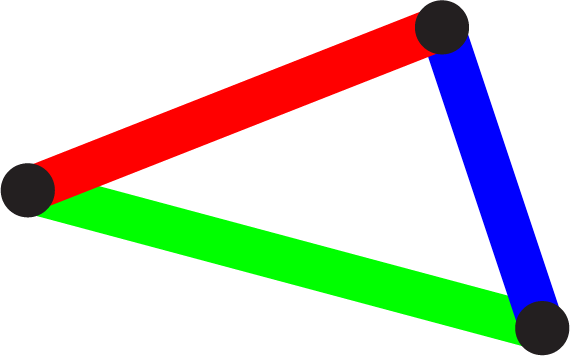
\includegraphics[scale=0.05]{Images/triangle_logo.png}}
}

\section{Background Theory}
Ray tracing is a family of techniques capable to perform an approximated light transport simulation to render an image, starting from a methematical representation of a scene. In order to simulate light transport, the main algorithm of any ray tracer consists of the following steps:
\begin{enumerate}
    \item Cast rays from the light sources present in the scene;
    \item For each ray, find the first collision with an object of the scene;
    \item Based on the material of the object, decrease the energy of the ray, and make it bounce to a different direction;
    \item This process is recursively carried out until the ray loses all its energy, or it hits the camera;
    \item If the ray hits the camera, color the hit pixel of its sensor based on the energy the ray is carrying.
\end{enumerate}

\begin{figure}[H]
    \centering
    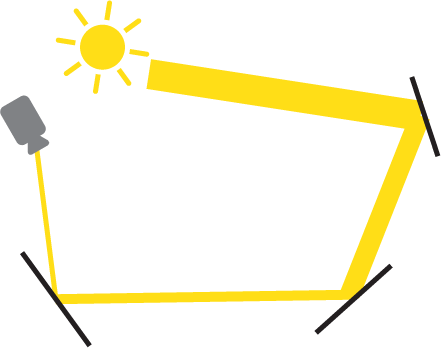
\includegraphics[width=\textwidth*\real{0.22}]{Images/ray_tracing_simple.png}
    \label{fig:ray_tracing_simple}
\end{figure}

Many of the rays cast from light sources end up not hitting the camera, therefore they are wasted. For this reason, in many ray tracing techniques the process is carried out in the opposite direction: the light rays are cast from the camera, and bounce around the scene until they hit a light source. These techniques fall under the name of backward ray tracing, and work thanks to the light reciprocity principle, which states that light transmit in the same way in both directions. From now on, when we refer to ray tracing, we implicitly reference backward ray tracing.

While ray tracing, at its core, is very simple, a lot of research effort has been put into making it faster. The main problem with light simulation is that, in the real-world, a huge amount of rays\footnote{A $100W$ lightbulb produces around $10^{20}$ photons per second.} are cast, in the form of photons, and are then captured by our eyes or a digital camera to produce an image. For this reason, one important family of optimizations has as main goal to reduce the number of rays needed to produce an accurate image.

\subsection{Kajiya and Monte-Carlo}
In order to understand better how these optimizations work, we first have to understand the Kajiya's rendering equation, which concisely describes how light transport work:

\begin{subequations}
    \begin{align*}
        L_o(\bar{x},&\bar{\omega}_o) = L_e(\bar{x}, \bar{\omega}_o) +\\
        &+\int_\Omega b(\bar{x}, \bar{\omega}_i, \bar{\omega}_o) \cdot \cos(\bar{n}, \bar{\omega}_i) \cdot L_i(\bar{x}, \bar{\omega}_i) d\bar{\omega}_i
    \end{align*}
\end{subequations}

In synthesis, this equation tells us that the amount of light exiting a poin $\bar{x}$ toward direction $\bar{\omega}_o$ is given by a constant emission term $L_e$, summed to a reflective term, decribed by an integral over an emisphere $\Omega$,

The integral term computes how much light the point $\bar{x}$ is receiving from all the directions of the hemisphere oriented toward the normal $\bar{n}$ to the surface the point is part of. Then, it uses the BRDF function $b$ to calculate how much of the light entering the point is reflected toward the direction $\bar{\omega}_o$.

The integral term is recursive, indeed, the light entering the point from a given direction $\bar{omega}_i$, corresponds to the light exiting another point.

\begin{figure}[H]
    \centering
    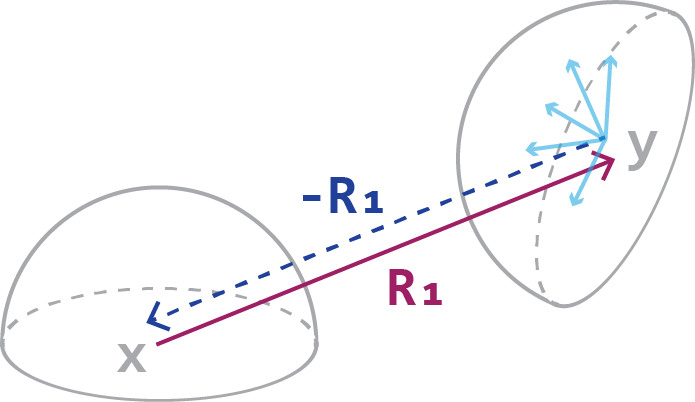
\includegraphics[width=\textwidth*\real{0.25}]{Images/kajiya_recursive.png}
    \caption{Recursiveness of the integral term.}
    \label{fig:kajiya_recursiveness}
\end{figure}

The task of any ray tracer is to numerically approximate the Kajiya's equation for any point of the scene, in order to, eventually, find out how much light each point reflets toward the direction of the focal point of the camera.

Computing the emissive term knowing where the light sources are located $L_e$ is trivial, the most time consuming part is to resolve the integral. In order to do so, Monte-Carlo integration is used. In this summary we assume that Monte-Carlo integration is known by the reader, and we focus mostly on how to apply it to the ray tracing context. In particular, to estimate the light entering the point hit by a view ray\footnote{An initial ray originating at the camera.}, we can cast a certain amount of probe rays toward random directions. The probe rays will hit another point, where othe probe rays will be cast, recursively, until the probe rays lose all their energy\footnote{In practice, after a certain recursion threshold.}, or they hit a light source.

The more probe rays we cast, the more the estimation of the light entering a point is accurate, and, consequently, the rendered image. The issue is that, by a fundamental Monte-Carlo estimator property, to cut the estimation error in half, we need 4 times more probe rays. For this reason, some variance reduction techniques have been developed to reduce error without increasing the number of rays.

The variance reduction technique important for this thesis is called importance sampling. Instead of casting the probe rays toward uniformly random directions, we cast them by following a non-uniform Probability Density Function (PDF). The PDF should be proportional to the integrand function but, since it is unknown, we can approximate it by casting more rays directly toward light sources. This importance sampling method is called light sampling, or Next Event Estimation (NEE).

NEE makes it so that the ray distribution inside the scene is not uniform, but it is more dense in proximity of light sources. This is a core hypothesis of our work.

\subsection{BVHs}
Until now, we have assumed we know where a ray intersect an object of the scene. In the real world, this is not the case, and finding the ray-scene intersection is a task common to any ray tracing algorithm. For this reason, the second big family of optimization is to find a way to accelerate this process. In the vast majority of graphics applications, the scene is described by a huge amount of triangles, approximating the surfaces of the objects. An object formed by triangles is called a mesh.

Therefore, the problem of finding the ray-scene intersection can be reduced to the problem of ray-triangle intersection, which has a known and very optimized solution. The first, naive, way of finding the intersection between a ray and the scene is a brute-force loop over all the triangles present in the scene. However, this method complexity increases linearly with the number of triangles or the number of rays in the scene. 

A better technique, which is used in state-of-the-art ray tracers, is to organize the triangles hierarchically, in a spatial binary tree called Bounding Volume Hierarchy (BVH). The idea is to divide the scene into two parts, and enclose the triangles inside each one into two parallelepiped aligned with the cartesian axes, called Axis-Aligned Bounding Boxes (AABB). Now, if a ray doesn't intersect an AABB, it won't intersect any of the triangles inside it, therefore AABBs can be used as rejection test. In a BVH this simple idea is applied recursively: the scene is divided into two AABBs, then each one is further divided into two, and so on, until a stopping criterion is met.

With a balanced BVH, finding the ray-scene intersection becomes logarithmic with reference to the number of triangles, and is therefore a big improvement over the brute-force approach.

Building the BVH optimally is an NP complete problem, therefore, in real-world applications, a greedy algorithm and heuristics are used to make the problem tractable. In particular, the heuristics are used to decide along which axis to cut the AABB, and to decide how to split the triangles into the two children nodes.

The first heuristic used in state-of-the-art applications is the Longsest Spliting Plane Heuristic (LSPH), where the AABB is cut with a plane perpendicular to its longest dimension. It is worth noting that, in all the state-of-the-art builders, only the three cartesian planes orientations are took into considerations. In other words, it is not possible to cut the AABB with an oblique plane, as it wouldn't make sense when the AABBs are, indeed, axis aligned.

The second heuristic is Surface Area Heuristic (SAH). With SAH, when the builder has to split the triangles by using the plane orientation selected by LSPH, it tries many different options\footnote{Binned approach.}, and assigns to each one a cost, which can be compute with this formula:

$$
Cost(Aabb) = \frac{SurfaceArea_{Aabb}}{SurfaceArea_{root}} \cdot \#triangles_{Aabb} \cdot K
$$

In summary, the formula tries to approximate the probability that the AABB is hit by a random ray, and weights it with the number of triangles in the node and a constant. The split with the lowest combined cost (i.e. hit probability) among the two AABBs gets greedly chosen.

The fact that the hit probability can be computed as $\frac{SurfaceArea_{Aabb}}{SurfaceArea_{root}}$ has as hypothesis that the rays are uniformly randomly distributed in the scene. However, as we noted while talking about importance sampling, we know this is not the case.

\section{Projected Area Heuristic}
The first novelty in our work is the Projected Area Heuristic (PAH). The core principle behind PAH is to try to estimate better the hit probability of an AABB, by leveraging the knowledge about the ray distribution in the scene, caused by light importance sampling.

In particular, we take into account two possible ray distributions:
\begin{description}
    \item[Parallel ray distributions] arise in proximity of planar area light sources;
    \item[Radial ray distributions] arise in proximity of point light sources, such as spotlights. 
\end{description}

\begin{figure}[H]
    \centering
    \subfloat[Parallel]{
        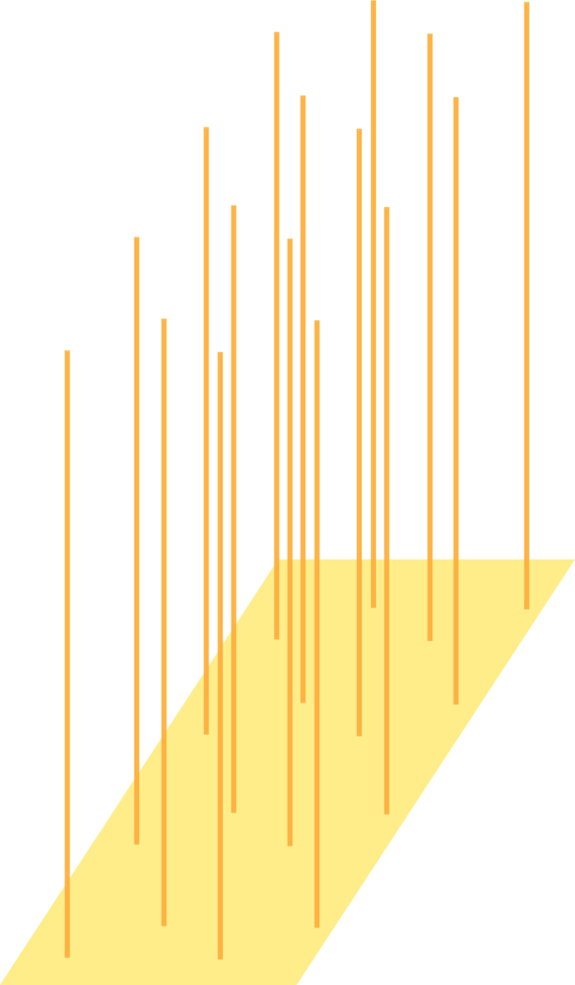
\includegraphics[width=\textwidth*\real{0.1}]{Images/plane_light_rays.png}
	}
	\qquad
	\subfloat[Radial]{
        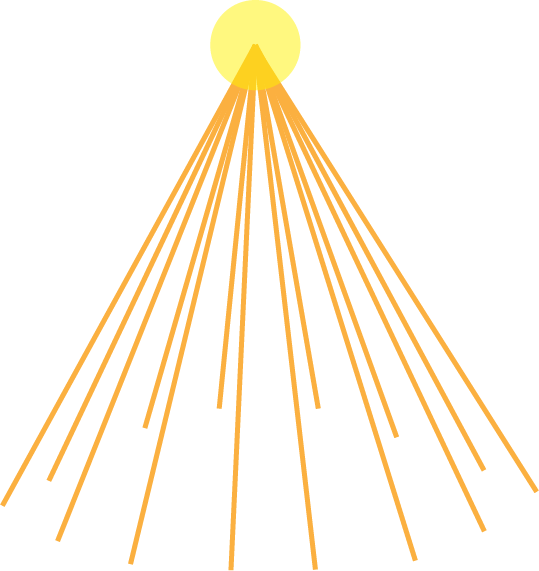
\includegraphics[width=\textwidth*\real{0.15}]{Images/point_light_rays.png} 
    }
    \label{fig:ray_distributions}
\end{figure} 

If one of these ray distributions is present in a given region of the scene, then we can better estimate the probability a ray hits an AABB present in this region, by projecting the AABB: in case of parallel ray, the projection is orthographic, whereas, for radial rays, the projection is perspective.

\begin{figure}[H]
    \centering 
    \subfloat[Orthographic]{
        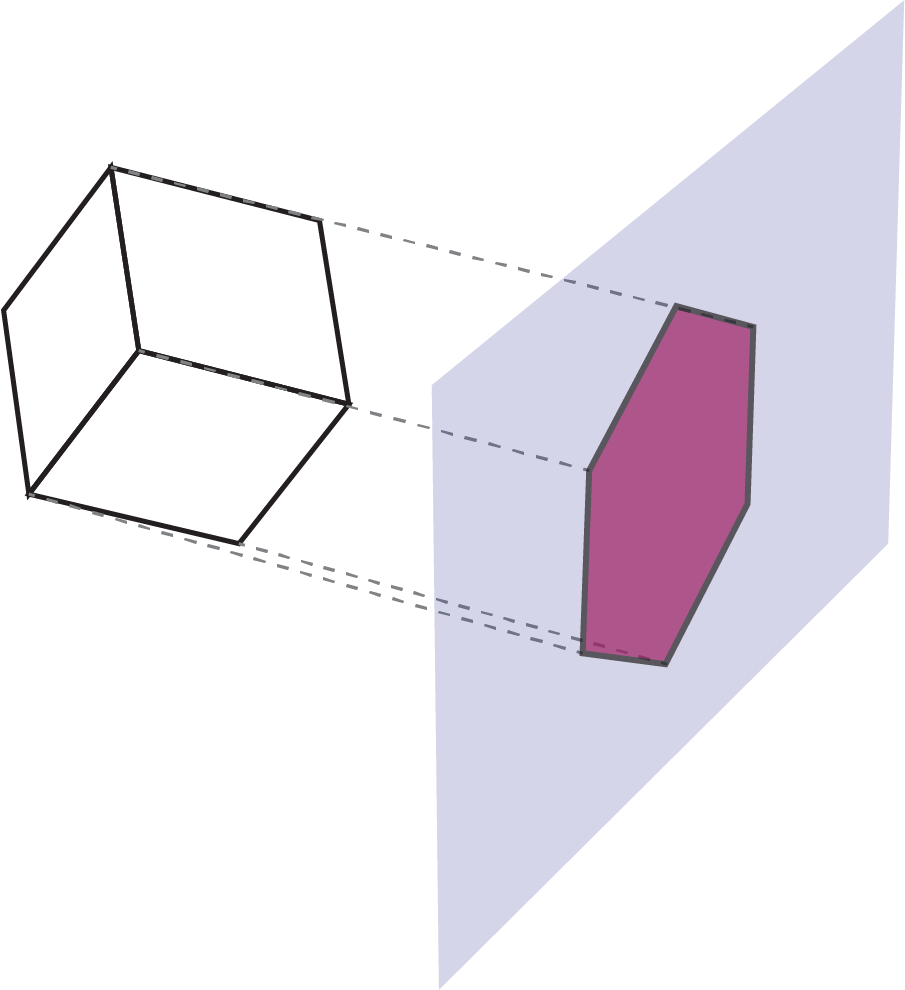
\includegraphics[width=\textwidth*\real{0.15}]{Images/ortho_projection.png}
	}
	\qquad
	\subfloat[Perspective]{
        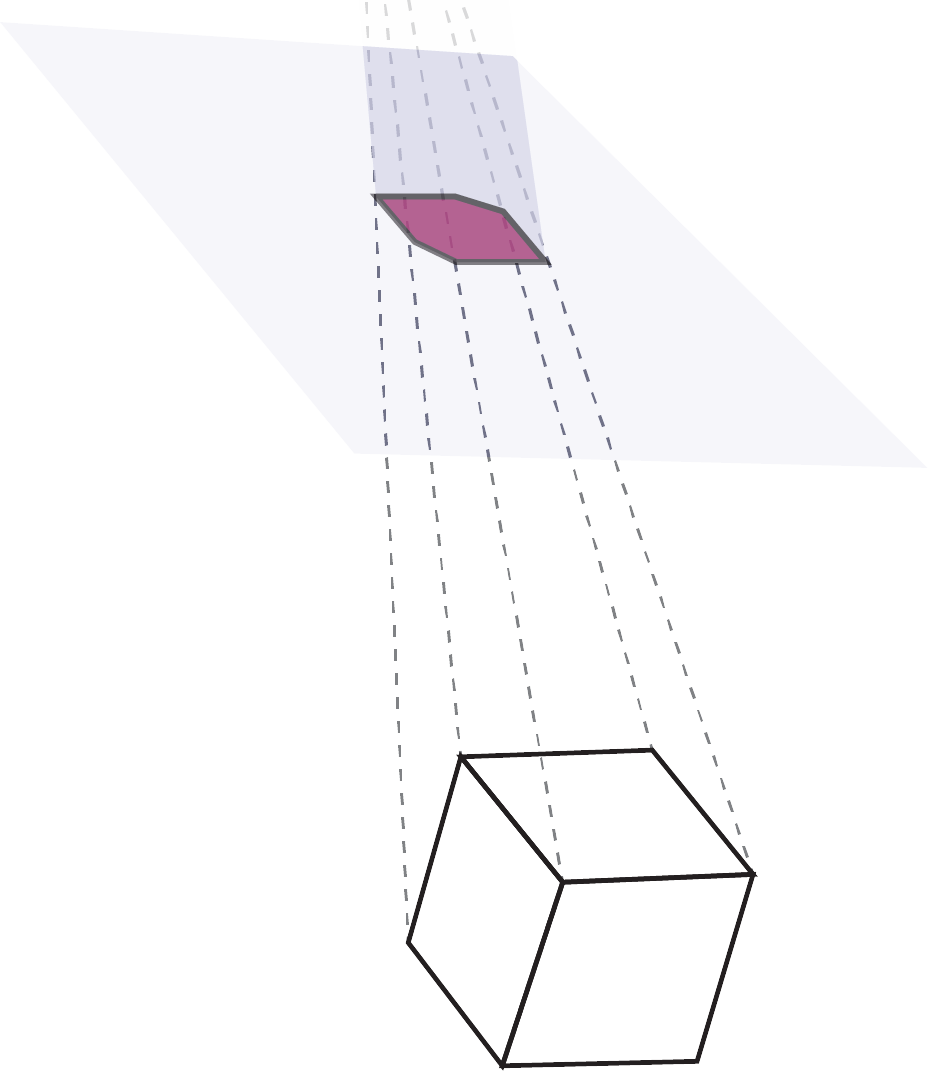
\includegraphics[width=\textwidth*\real{0.15}]{Images/perspective_projection.png} %TODO improve image
    }
    \label{fig:projections}
\end{figure}

\section{Splitting Plane Facing Heuristic}
The second novel heuristic we propose, is a possible alternative to LSPH, and is called Splitting Plane Facing Heuristic (SPFH). It is based on the same considerations we made for PAH, but it is applicable to how to decide the orientation of the splitting plane, and takes into consideration if the AABB is in a region with a parallel or radial ray distribution.

As described by \cite{bvh_overlapping_metric}, a big 3D overlap between two children nodes, leads to a low quality BVH. With SPFH, we try to minimize the overlap between children nodes in the 2D space of their projections. The idea is based on the observation that, if the splitting plane is perpendicular to a ray, there is a large probability that the ray will intersect both the resulting children AABBs. Conversely, if the plane is parallel to a ray, it is not probable that it will hit both, because the overlap of their projections will be a lot smaller in many scenarios.

\begin{figure}[H]
    \centering 
    \subfloat[Perpendicular]{
        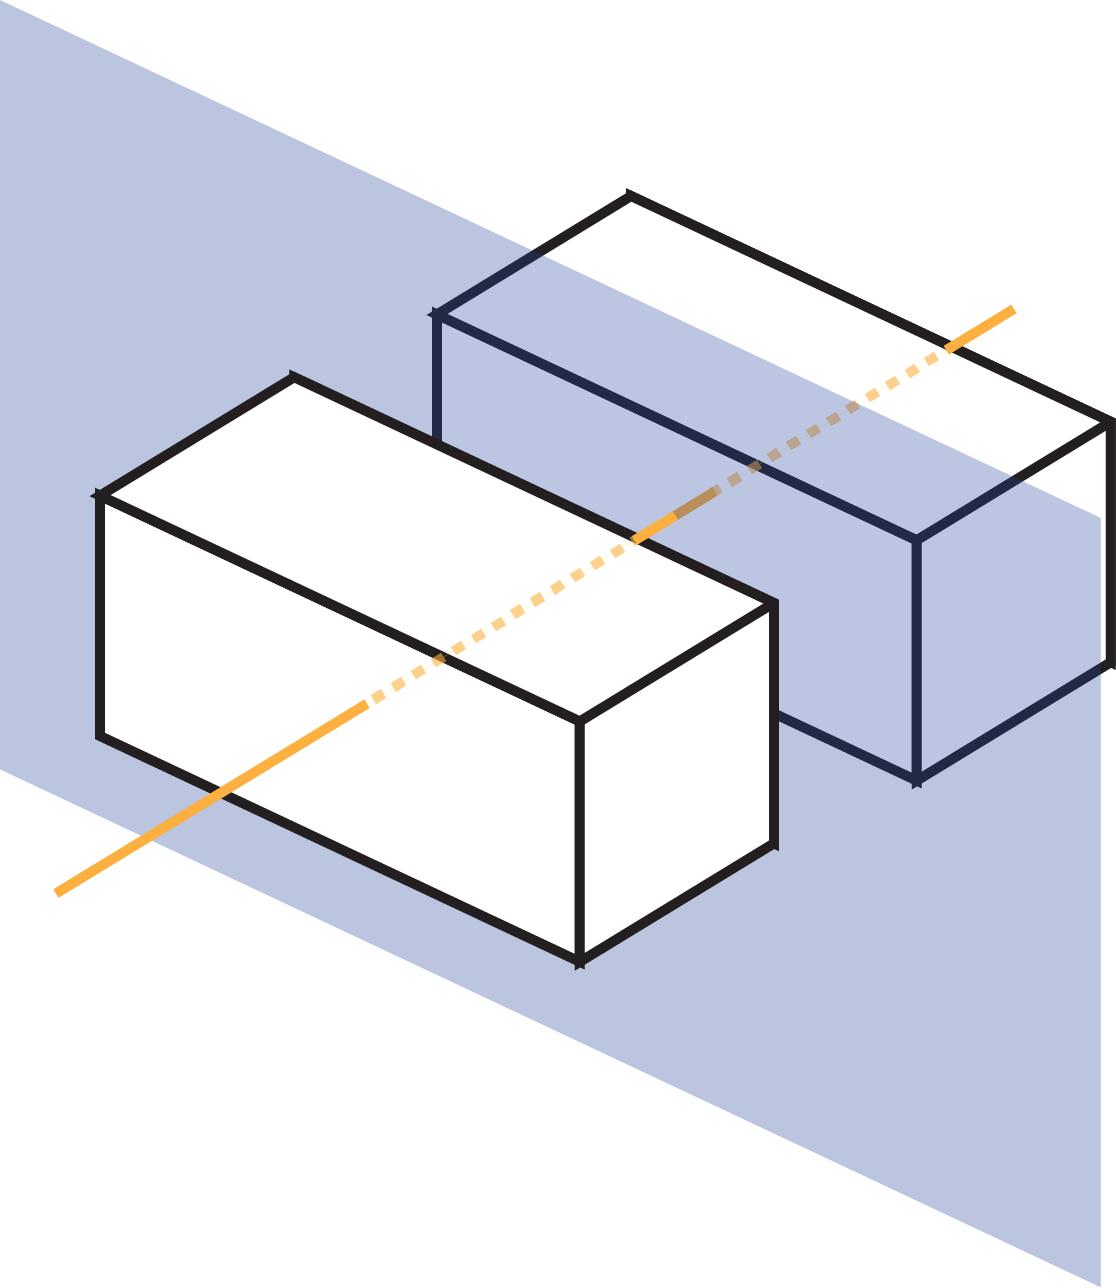
\includegraphics[width=\textwidth*\real{0.15}]{Images/z_axis_plane.png}
	}
	\qquad
	\subfloat[Parallel]{
        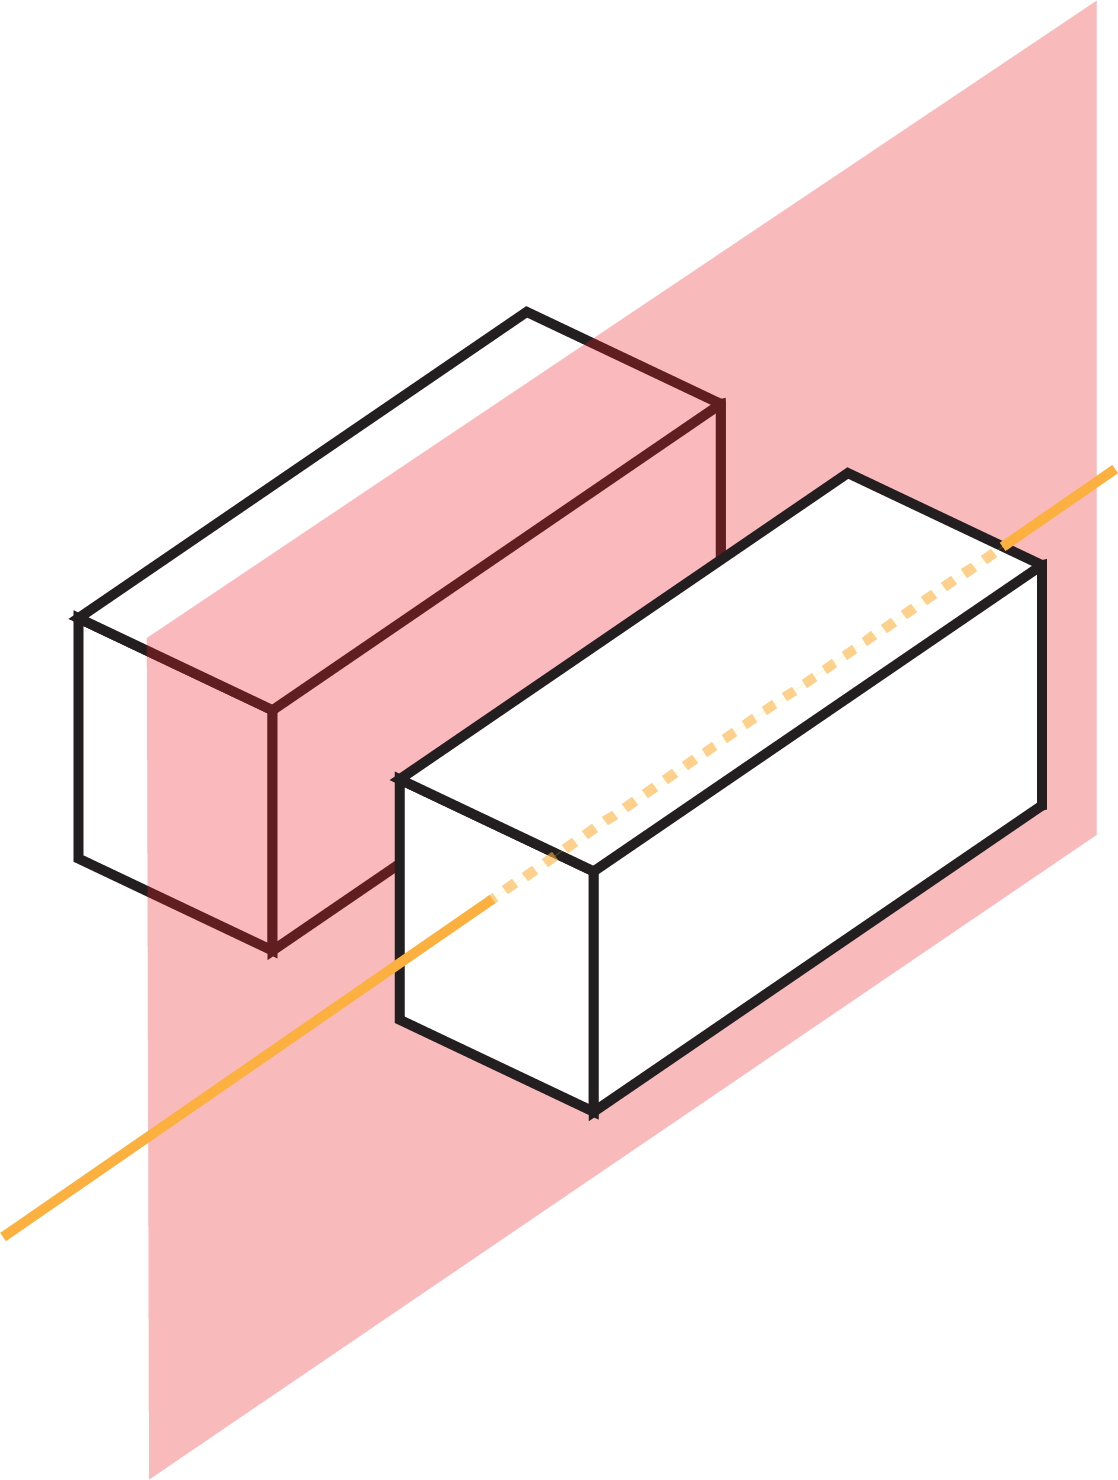
\includegraphics[width=\textwidth*\real{0.15}]{Images/x_axis_plane.png}
    }
    \label{fig:splitting_overlap}
\end{figure}

In our implementation, better described in the relative section, for each one of the possible three splitting planes orientations, we assign a value which tells the builder how much parallel a plane is to the rays of the ray distribution the AABB is placed into. The builder will then try the splitting plane with the highest value, and use PAH to find the actual best cut.

\section{Top Level Structure}
In the previous sections we summarized the two novel heuristics we propose. In this section, we will introduce two structures that can be used to enable the adoption of our heuristics in a concrete case.

% === Bibliography ===
\bibliography{../Thesis/bibliography.bib}

\end{document}